\chapter{Background}
\label{chap:background}

This chapter presents background information about interdomain routing, the
CIDR Report, and Internet coordination and operations that will be useful in
providing conceptual and historic context about a number of the aspects of this
thesis. The first section, which contains a primer on interdomain routing, is
provided as a guide to the reader in order to discuss and articulate a number
of the technical features of Internet routing and operations that are crucial
to understanding this thesis and which are relied upon extensively in the
approach used to answer the thesis question. Advanced readers may wish to skip
ahead to the second and third sections, focused on the CIDR Report and Internet
coordination respectively, which contain much more specific background
information relevant to the this thesis that may not be widely known.

\section{Routing and Internet operations}

Interdomain routing (IDR) is essential to both the concept and operation of the
Internet as a ``network of networks''. IDR enables the multitude of privately
owned and operated networks that exist around the world to connect and exchange
reachability information, which in turn enables a host connected in one network
to contact another host connected to any other network. In the context of
today's Internet, IDR is used to establish the topological location of blocks
of network-layer identifiers---IP addresses---as well as routes to these
blocks. This information allows routers within each network to send traffic
destined for other networks in the appropriate ``direction'' in order to reach
that network. The set of possible routes available for traffic from a network
will be constrained by connectivity to other networks, as well as the
commercial interests of Internet service providers who desire to route traffic
to earn revenue or reduce costs.

This section begins with a broad overview of some of the fundamental aspects of
IDR and the provision of Internet service from both a technical and a
commercial perspective. From this foundation, the specific details of the
Internet routing table and the protocol, BGP, used to establish it are
discussed. Finally, commonly-used Internet operations activities that utilize
BGP and thus affect the routing table are discussed.

\subsection{Interdomain routing}

The interconnection of diverse networks was the fundamental design goal of the
Internet \cite{Clark:1988kl}. While this goal prompted a number of design
decisions that have resulted in the Internet as we know it today, the
Internet's system of interdomain routing is one of the key operational
components for realizing this goal.

Routing generally refers to the process by which paths to specific destinations
are determined, as well as the forwarding of incoming packets along the the
previously-determined best path towards the ultimate destination. Each router
need not know the entire path to every other destination on the network; the
router simply passes the packet along to the next hop that has indicated that
it knows the way to the destination. In this context, a route can be considered
abstractly as a claim that the router announcing a route knows of a path that
should deliver a message to a given destination, and is willing to deliver it
to the next closest point in the path that it knows of.

Routing takes place at two scopes in networks today. First, \emph{intradomain}
routing takes place within networks, the boundaries of which are typically
demarcated by infrastructure ownership or policy (e.g. a business or campus
network). Routes are typically established using dynamic interior routing
protocols such as OSPF or IS-IS. The goals of interior routing are mainly to
establish network-wide reachability efficiently, with little concern about the
path taken. The presence of a route simply means that a link is up and can
carry traffic. Operators may adjust link metrics to balance traffic flow across
networks, but there are not many other concerns about which parts of the
network know about or utilize which routes.

The second scope is between networks, such as the multitude of networks that
interconnect to make the Internet. Unlike intradomain routing,
\emph{interdomain} routing is focused on exchanging reachability information
between various networks that are owned and operated with different policies
and objectives. While reachability is still an important concern, other
concerns relate to routing policy---the expression of desired behavior for
network traffic. Routing policy is typically motivated by business concerns
ultimately related to the carriage of traffic. In the context of interdomain
routing, the exchange of routing information with another domain indicates a
willingness to carry traffic to the route's destination. Thus, control of route
announcements is important for business reasons. Routing policy objectives also
include selective route advertisement in order to control traffic flow, as well
as finer-grained capabilities to govern where traffic enters and exits a given
network.

On the Internet, interdomain routing information is exchanged between
\emph{autonomous systems} or ASes. These represent domains of consistent
routing policy \cite{rfc1930}, and typically consist of a single organization's
network, though complex network designs sometimes organize an organization's
networks into multiple ASes for various reasons. Each AS is identified by a
unique number, an AS Number, assigned to it by the Internet Assigned Numbers
Authority (IANA) or the appropriate Regional Internet Registry (RIR). These
identifiers are used as short-hand operational handles to refer to networks:
MIT holds AS number 3, and AT\&T's North American backbone is often referred to
as ``AS 7018''.

With the notions of routes and autonomous systems defined, we can consider that
the Internet abstractly as a directed graph with ASes as vertices and edges
representing the willingness to carry traffic (according to the advertised
routes) for adjacent ASes. Let us now consider what the incentives are for ASes
to interconnect, and the types of relationships this forms between networks as
a result.

The value that comes from interconnecting networks is a sort of network
effect---like other forms of communication, the Internet's value increases as
the number of hosts reachable via the Internet increases. It is a long standing
tradition on the Internet for pairs of networks that receive mutual benefit
from interconnecting to do so without charging the other for the traffic sent.
This practice is known as peering, and the pair of connecting networks would be
considered to have a peer relationship. Peering is effective when the
interconnecting networks derive similar benefits from the interconnection and
when they are directly adjacent, but this is not often the case in the
Internet. Unlike the case where peers gain benefit from connecting and
providing access to each others users/customers, peers do not benefit when they
carry traffic between two other peer ASes connected to it---what is known as
providing \emph{transit} for those two networks. A different approach is
required for networks that do not connect directly but that still wish to reach
each other via the Internet.

Generally speaking, there are two ways for an autonomous system to receive
routes that enable them to access the rest of the networks that compose the
Internet. First, ASes may pay the other networks that they connect with to
carry traffic to and from the rest of the Internet on the AS' behalf. Payment
makes the carrying of traffic for others beneficial to interconnecting networks
in cases where it normally was not in the previous discussion of peering. In
these cases, the paying AS is a transit \emph{customer} of their upstream
networks. Alternately, an AS operator can build its own network to have
sufficient geographic breadth and presence in order to directly connect to
other networks. This is a capital-intensive operation and so these networks are
usually operated as businesses---network service \emph{providers}---to provide
transit service to other networks seeking connectivity to the Internet.

Each autonomous system is free to interconnect and exchange routing information
with other networks as they choose, and many have their own unique policies in
this regard. However, the generally-accepted logic is that routing policy is a
rational decision-making process with the goal of maximizing income and
minimizing payment. This can be distilled into a simple set of ordered
preferences for selecting routes within a given AS. To reach a given prefix
from a given AS, routes are preferred in the following order of availability:

\begin{enumerate}
    \item{Prefer a customer's route, as this allows the AS to charge the
    customer for this traffic.}
    \item{If a customer route is not available, prefer a peer's route as this
    allows the AS to send the traffic without charge.}
    \item{If a customer or peer route is not available, use the upstream
    provider's route. This is the route of last resort, as the AS must pay its
    provider for this traffic.}
\end{enumerate}

The upstream provider route is usually installed as a ``default'' route, which
means it matches any prefix that the AS does not have specific routing
information about, on the assumption that the upstream provider has better
connectivity to other networks than the AS. This is a reasonable assumption,
especially for smaller networks at the edge of the Internet, and necessarily
true for those that obtain Internet connectivity from a single provider.

There is a small set of networks that are sufficiently large that they achieve
reachability to all other Internet networks by using customer and peer routes.
These networks are large providers that have many customers of their own, and
would never be customers of other large networks. This results in peering
relationships with their other large counterparts in order to reach the rest of
the Internet. These networks do not have default routes, and are thus
collectively known as the default-free zone (DFZ). The DFZ represents the
``core'' of the Internet, and its members have the most complete view of the
Internet and play a significant role in Internet routing.

\subsection{The Border Gateway Protocol}

The Border Gateway Protocol (BGP) is the standard interdomain routing protocol
that runs between networks to achieve Internet connectivity. The BGP
specification defines a protocol for exchanging reachability information
between autonomous systems, as well as an algorithm for selecting paths and
means for expressing routing policy based on path advertisement and selection.

BGP operates as a bilateral session established between two BGP-speaking
routers in adjacent autonomous systems. Once the session is established,
network layer reachability information---IP address prefixes---that are known
to each router is transmitted to the other AS' router, along with attributes
corresponding to the prefixes, such as the origin, AS\_PATH, or the IP address
of the next hop router for packets destined for a prefix. The routes
advertised to one's neighbors may either originate from within the AS (for
customers and infrastructure) or be from  other neighbors that one agrees to
provide connectivity for. As the paths to prefixes change (such as when a link
comes up or goes down), or as new prefixes are advertised or become
unreachable, update messages are sent advertising or withdrawing routes
accordingly. As route updates are received, the router updates its routing
information base and may select and advertise a new best path based on this
change in information.

The AS\_PATH feature of BGP is a distinguishing characteristic of the protocol
and one of the most relevant characteristics of the protocol for the purposes
of this thesis. It is constructed as announcements are received and
re-announced by autonomous systems providing transit to each other. Each AS who
announces a route appends their AS number to the AS\_PATH of the prefix. This
serves to provide loop prevention, as BGP speakers ignore routes with their own
AS in their AS\_PATH. The AS\_PATH also serves as a source of topological
information, identifying the AS that first announced the prefix---the origin
AS---as well as the vantage point AS and the ASes in between.

An illustrative example of a BGP route announcement and corresponding topology
that generates the AS\_PATH is shown in Figure \ref{fig:bgp_announcement}.
Looking at the AS\_PATH in the update message, we can see that the prefix was
originated by MIT (AS 3), observed by Route Views peer Phonera (AS 16150) and
transited by MIT's upstream provider Sprint (AS 1239) and intermediate provider
Global Crossing (AS 3549). In this case Route Views (AS 6447) is the vantage
point and so its AS number is not recorded in the AS\_PATH. By observing the
AS\_PATH information contained in a diverse set of routing tables, such as is
visible from Route Views \cite{Routeviews}, a great deal of information about
connectivity and topology can be gathered.

\begin{figure}
\begin{centering}
    \subfigure[An example BGP topology showing AS relationships (black edges)
        and BGP route announcement progression (red edges).]{\raisebox{-0.5in}{
        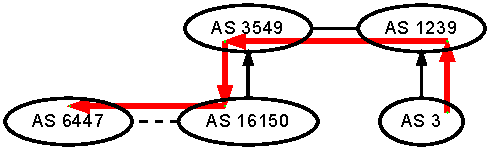
\includegraphics{figures/bgp_example_topology_fixed.pdf}}
        \label{fig:bgp_announcement:topology}}
    \subfigure[An example route advertisement (UPDATE) message received by AS
        6447 reflecting the topology in \ref{fig:bgp_announcement:topology}.]{
        \small{
        \begin{tabular}{| c |}
        \hline
        \textbf{UPDATE}\\
        \hline
        \multicolumn{1}{|l|}{\emph{path attributes=}}\\
        AS\_PATH: 16150 3549 1239 3\\
        NEXT\_HOP: 217.75.96.60\\
        \ldots\\
        \hline
        \multicolumn{1}{|l|}{\emph{prefixes=}}\\
        18.0.0.0/8\\
        \ldots\\
        \hline
        \end{tabular}
        }
        \label{fig:bgp_announcement:update}
        }
    \caption{A simplified BGP topology and corresponding route announcement.}
    \label{fig:bgp_announcement}
\end{centering}
\end{figure}

%\fbox{figure of route announcement}
%\begin{verbatim}
%	route-views>show ip bgp 18.0.0.0/8
%	BGP routing table entry for 18.0.0.0/8, version 5243
%	Paths: (38 available, best #34, table Default-IP-Routing-Table)
%	...
%	  16150 3549 1239 3
%	    217.75.96.60 from 217.75.96.60 (217.75.96.60)
%	      Origin IGP, metric 0, localpref 100, valid, external
%	      Community: 3549:2773 3549:31208 16150:63392 16150:65321 16150:65326
%	...
%\end{verbatim}

% While generally not relevant to this discussion, BGP specifies a
% decision-making algorithm and tie-breaking procedure for consistently
% selecting the best path to a given prefix. What is perhaps important to note
% is that for forwarding traffic (as opposed to route selection), the most
% specific prefix that matches a given IP address will always take precedence.
% This is necessary to allow for subnetting---the specification of more
% specific networks with different routing policy than the covering parent
% address block---but this property also facilitates route hijacking. Both of
% these issues are discussed later in this section.

Routing policy can be controlled and expressed in a few ways with BGP.  First,
route advertisements incoming from neighbors may be filtered to ensure that the
routes accepted into one's own routing table agree with business and
operational practices. Similarly, outgoing route advertisements to neighbors
may be filtered to ensure that routing policy is maintained (such as not
providing transit to peers). Finally, operators may tag their outbound route
announcements with BGP Communities. These are (generally) provider-specific
attributes that affect the way providers will treat route announcements they
receive, such as prepending the route's AS\_PATHs or announcing the route to
only part of their network. There are a few well-known community attributes
that are defined in the RFCs \cite{rfc1997}, including the NO\_EXPORT
attribute, which should instruct a peer to not share (export) the prefix with
any of its neighbors.

\subsection{The Internet routing table}

The Internet routing table is where global Internet reachability information is
collected and maintained by each autonomous system. Each AS will construct
their routing table based on connectivity with their neighbors and their
own routing policy objectives. The Internet routing table can be constructed in
a number of ways, including the manual configuration of routes by a router
operator, but it is most commonly constructed by running BGP with one's
neighbors to exchange reachability information.

While it's commonly referred to as \emph{the} Internet routing table or the
\emph{global} routing table, there is no canonical definition of the routing
table. Each AS will have its own unique view of the Internet through its
routing table because of that AS' unique position in the topology of the
Internet. The AS' own policy requirements, as well as the routing policies of
its neighbors will also affect the set of routes that it observes relative to
other vantage points on the Internet. However, most ASes will have a roughly
similar view of the Internet.

The Internet routing table is implemented as two sets of related data in most
routers and as used by most networks. The main table of Internet routing
information in an interdomain router is more precisely defined in the BGP
specification \cite{rfc4271} as the routing information base (RIB). Many
routers also maintain a forwarding information base (FIB) as described below.
All feasible routes received over all BGP sessions are stored in the router's
RIB and remain there unless updated or withdrawn at a later time. The RIB may
contain multiple possible routes for a given destination, and so cannot be used
directly for forwarding packets. Instead, the BGP path selection algorithm is
run over the data in the RIB to select the best path for each prefix. These
best paths are then installed in the FIB where they are then used to forward
packets to neighboring networks in order to reach their final destination.
These best paths are also exported to any peers and customers of the AS, after
filtering to enforce routing policy.

The FIB is typically a more compact version of the best paths in the RIB, and
resembles a lookup table within each AS' border router that is used to
determine the link along which incoming packets should be forwarded in order to
reach the destination as specified in their IP packet header. An excerpt
illustrating what a routing table might look like is shown in Figure
\ref{fig:ex_routing_table}.

\begin{figure}[h!]
    \begin{center}
    \begin{singlespace}
    \small
        \begin{tabular}{c | c | c}
            \textsc{prefix} & \textsc{next hop} & \textsc{interface} \\
            \hline
            ... & ... & ... \\
            10.0.0.0/8  & 192.168.10.1   & eth0 \\
            10.1.0.0/14 & 172.16.120.200 & eth1 \\
            10.2.1.0/24 & 172.16.120.204 & eth1 \\
            ... & ... & ...
        \end{tabular}
    \end{singlespace}
    \end{center}
\caption[A partial example of a routing table]{A partial example of a routing
table showing next IP hop, and physical egress interface for each prefix.}
\label{fig:ex_routing_table}
\end{figure}

For each incoming packet, the router searches the table for the most specific
(longest) prefix that matches the destination address and forwards the packet
to the router specified by the address in the ``next hop'' column of the table.
In the example above, a packet destined to 10.1.2.3 would be forwarded to the
router at 172.16.120.200 over the `eth1' interface.

The resources within routers that are used to store the RIB and FIB and execute
the BGP route selection algorithm are generally finite and fixed by the design
of a given router. The RIB is stored in a router's route processor DRAM, and
the route processor CPU executes the BGP path selection algorithm on receiving
a BGP update message from a peer. These routes are then installed in the FIB,
which is copied to high speed lookup memory (often content-addressable memory)
associated with special packet forwarding processors on router linecards
\cite{Zhao:2010fu}. Given these limits, the scalability of the Internet is
constrained to some degree by how its growth affects the size of the Internet
routing table. The upper ceiling on router memory limits the absolute growth of
the routing table in terms of the number of routes it can maintain. Each entry
in a router's routing table memory is often colloquially referred to as a
``slot''.

While this memory limitation is less of a problem in modern routers with
multi-gigabyte memories and multi-million route capacities, this was a
significant problem in early routers as the Internet began growing quickly in
the early 1990s, with routers failing or behaving unusually as the routing
table consumed all available memory \cite{Li:2011vn}. In contrast, router CPU
utilization poses less of an absolute limit on routing table growth, but does
cause other challenges. As the size of the routing table grows, the amount of
data required to be processed for a large routing update or BGP session startup
or reset has become significant. It is apparently not unusual for this initial
router startup process to take tens of minutes \cite{Steenbergen:2010nx} before
routes are exchanged with peers and connectivity is fully established. More
generally, as the time required for processing routing updates increases, the
time for routes to converge after a BGP update will also increase, resulting in
poor performance and potential partial loss of Internet connectivity during
transient network failures. Concerns over the stability and scalability of
Internet routing has made the growth of the routing table and BGP UPDATE
dynamics a topic of interest for at least the past two decades.

\subsection{Routing policy and BGP network operations}

At its simplest and most efficient, the Internet routing table should contain
one entry per autonomous system. Given that there are approximately 40,000
autonomous systems visible on the Internet today, this would yield a small and
compact routing table, similar to that of the mid-late 1990s. However, the
routing table cannot be made that simple for a number of reasons. The
needs-based allocation policies used by RIRs \cite{rfc2050} to allocate blocks
of IP addresses to end-user organizations results in fragmentation of IP
address blocks and allocation of non-contiguous blocks to organizations as they
receive new addresses over time. Such blocks cannot be announced as a single
prefix, and so multiple routing table slots must be consumed to advertise each
disjoint block allocated to an organization. Beyond fragmentation, most cases
of increased consumption of routing table slots are the result of implementing
routing policy for traffic incoming to a particular AS using the mechanisms
available in BGP. A number of these mechanisms are discussed in turn below.

Control of routing policy for traffic exiting an AS is relatively
straightforward---the AS operator simply needs to express and adjust their
preferences for which route of those that they receive from their peers,
customers, and providers should be selected for carrying that traffic to the
specified prefix. In contrast, managing routing policy for traffic entering an
AS is much more difficult because selection of the best path for traffic
originating from all other networks occurs independently in each remote network
and is dependent on factors such as AS\_PATH length that the AS advertising a
route lacks control over.

Many of the operational requirements of network service providers today
for control over inbound traffic are not directly facilitated by explicit
BGP features. Indeed, BGP provides only one ``knob'' that an AS operator can
adjust to influence its adjacent peers' path selection: the relatively limited
multi-exit discriminator (MED) attribute \cite{Beijnum:2002oq}. To achieve
desired routing policy in more advanced situations such as multihoming and
traffic engineering, operators must implement routing policy using other
aspects of the BGP protocol. By understanding how the BGP path selection
algorithm works and assuming that most peers follow the standard algorithm, an
operator can implement more effective and fine-grained routing policy.

It is important to note that in general, each of these behaviors allows an AS
to obtain private benefit by imposing a public cost against all other
participants in the global routing system. To announce a multihomed or traffic
engineered network, which provides benefit to the operator initiating that
behavior by allowing them to better manage their network, they necessarily add
extra routes to the routing table of every network operator that collects a
full routing table from their peers.

\paragraph{Multihoming}

Multihoming refers to the connection of a network to the Internet via more than
one upstream provider. This is typically motivated by a desire for reliability,
such that one will have network connectivity even in the event of a failure or
misconfiguration on the part of an upstream provider. A basic approach to
establishing connectivity for a multihomed AS would be to announce all of the
AS' prefixes to all of the AS' upstream providers (sometimes referred to as
anycasting). Depending on one's view of the Internet, a slot in RIB may be
consumed for each of these announcements (i.e. for each of the upstream
providers).

This will achieve the goal of multihoming, but may result in an imbalance of
traffic between upstream links as distant ASes select the path to take based on
factors that the origin AS likely does not have control over, such as the
AS\_PATH length. This can pose a problem if the AS' primary link is inexpensive
and the backup link is expensive. The typical approach used to solve this
problem is called AS\_PATH prepending, where an AS will artificially lengthen
their AS\_PATH as observed by certain (e.g. high cost) providers in order to
make specific links less attractive for incoming traffic. Other issues
regarding balance over links may arise, and these are best handled by the
general class of behavior called traffic engineering.

\paragraph{Traffic engineering}

Traffic engineering (TE) refers to balancing traffic across network links to
avoid overloading particular links (resulting in high latency and potentially
loss) and allowing headroom in a given link's utilization to allow for bursty
traffic. TE is easy to perform for traffic leaving an AS with multiple upstream
links, as the AS operator has control over their interior routing protocol
metrics and their border routers themselves, and can thus direct traffic as
they wish. Inbound TE is more difficult, again because of the lack of knobs
that an operator has to select the ingress point for inbound traffic into their
network.

While AS\_PATH prepending and the MED can both be used effectively for inbound
traffic engineering sometimes, the ultimate tool for fine-grained TE is the
announcement of more-specific prefixes. Because the BGP path selection
algorithm always prefers more specific prefixes, a network operator can
distribute high-traffic destinations within their network across multiple
prefixes or subnets within their prefix and announce these more-specific
prefixes separately to their various peers and upstream providers in order to
spread incoming traffic across multiple incoming links. Each of these
more-specific prefixes generally cannot be aggregated with the less
specific-covering prefix because the routing policy differs (the AS\_PATHs will
likely be different because of the selection of different upstream providers
for different prefixes).

% In some cases, TE is difficult to discern between providers

% BGP network operations that affect the Internet routing table - poor
% advertisements - multihoming and traffic engineering - anycast - path
% prepending - cut-outs/more-specifics - hijacking prevention - prefix length
% filtering (and impacts on reachability therein)

\paragraph{Prefix hijacking prevention}

Prefix hijacking is the announcement of an IP address block by a network other
than the legitimate owner of an address block. This can sometimes result from
configuration errors \cite{Brown:2008hc} but can also be an intentional attack
against a network \cite{Pilosov:2008ij}. These attacks are particularly
effective because routes with the longest matching prefix are selected,
allowing the most specific prefix to ``win'' the traffic, even if its path is
less optimal. To guard against the hijacking of address blocks, particularly
for critical infrastructure such as authoritative name servers, some providers
announce parts of their address blocks with the most specific prefix that they
expect will be successfully pass global route filtering policy. This typically
leads to the advertisement of /24 blocks for critical
infrastructure\footnote{As a current example that is accurate as of the date of
submission of this thesis, Google.com locates its authoritative DNS nameservers
(e.g. ns1.google.com, which resolves to 216.239.32.10) in 216.239.32.0/24 and
other /24 blocks, advertised separately in addition to the covering
216.239.32.0/19 block allocated by ARIN.}.

%\begin{verbatim}
%> dig +short google.com NS
%ns1.google.com.
%
%> dig +short ns1.google.com A
%216.239.32.10
%
%route-views> sh ip bgp 216.239.32.10
%BGP routing table entry for 216.239.32.0/24, version 360859
%...
%
%route-views>sh ip bgp 216.239.32.0/24 shorter-prefixes
%...
%   Network          Next Hop            Metric LocPrf Weight Path
%*  216.239.32.0/19  194.85.102.33                          0 3277 15169 i
%...
%\end{verbatim}

\section{CIDR-ization of the Internet and the CIDR Report}

This section offers a mainly-historic background on an effort called classless
interdomain routing (CIDR) to allow more efficient announcement of address
blocks in the Internet's interdomain routing system. This section also provides
background and history on the CIDR Report, a social mechanism used to encourage
network operators to aggregate their route advertisements using CIDR.

\subsection{Classless interdomain routing}

In contrast to individual end hosts connected to an IP network, which are fully
identified by an IP address, there is also the need to refer to
\emph{networks}---collections of hosts connected together in such a way that
they are all reached by the same path. In other words, networks are blocks of
IP addresses that have the same routing policy and are thus reached in the same
way. An IP address contains both the network address and the subnetwork address
of that machine on the given network. The differentiation between the network
and the subnetwork is given by partitioning the 32-bit IP address into a
network part and subnet part, as shown in Figure \ref{fig:ip_prefix_address}.
Networks are a useful abstraction in interdomain routing in that they allow
routers to maintain a relatively small amount of state to reach a potentially
large number of IP addresses, rather than maintaining routing information
separately for each Internet-connected host.

\begin{figure}[h]
\begin{centering}
    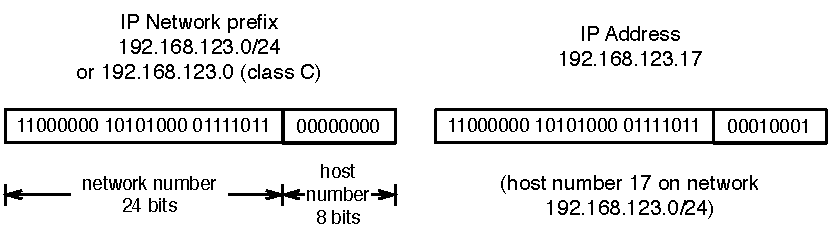
\includegraphics[width=6in]{static_figures/prefix_address.pdf}
    \caption[An example of an IP network prefix and a full IP address]{An
    example of an IP network prefix and full IP address, illustrating the
    distinction between the network number and host number components of the
    address. Note that the prefix length (e.g. /24) indicates the position of
    the partition between the network number and the host number, and thus the
    number of bits allocated to each.}
    \label{fig:ip_prefix_address}
\end{centering}
\end{figure}

The original specification of the Internet Protocol implicitly encoded the size
of the network in the first octet of the network address itself. Three classes
were available: class A, for large networks ($2^{24}$ hosts), class B, for
mid-sized networks ($2^{16}$ hosts), and class C for small networks ($2^{8}$
hosts).  Networks with the first octets shown in Table \ref{tab:addressing}
were assumed to be members of the class and thus be of that size. The
distribution between class A, B, and C networks was specified arbitrarily by
the protocol developers.

\begin{table}[h]
\begin{centering}
\begin{singlespace}
\small
\begin{tabular}{ c | c | c | c }
    \textsc{Class} & \textsc{Address Range} &
    \textsc{Hosts/Network} & \textsc{Networks/Class} \\
    \hline
	A & 0.0.0.0--127.0.0.0         & $2^{24}$ & $2^{7}$ (128)              \\
	B & 128.0.0.0--191.255.0.0     & $2^{16}$ & $2^{14}$ (16384)           \\
	C & 192.0.0.0--223.255.255.0   & $2^{8}$  & $2^{21}$ (2097152)         \\
	D & 224.0.0.0--239.255.255.255 & \multicolumn{2}{c}{multicast (224/4)} \\
	E & 240.0.0.0--255.255.255.255 & \multicolumn{2}{c}{experimental (240/4)}
\end{tabular}
\end{singlespace}
\end{centering}
\caption[Classful IP addressing architecture]{Classful IP addressing
architecture \cite{rfc791}}
\label{tab:addressing}
\end{table}

Assignment to permit use of these addresses by organizations was performed by
the IANA, and addresses were allocated on a basis of justified need. Large
organizations (e.g. MIT, General Electric, etc.) typically planned to, or were
assumed to have large networks and many hosts, and so were granted class A
addresses.  Organizations that were somewhere in the middle would be granted a
class B, and organizations expecting to have less than 254 hosts would get a
class C. As networks grew, they would often be assigned new blocks rather than
trading up to a larger block size---this was particularly frequent in the class
C space.  This issue of granting new class C blocks was also exacerbated by the
realization that the class B block was the most commonly needed network size,
yet was under-allocated compared to class C networks. As ASes with class C
blocks needed to grow, they were allocated multiple class C blocks to conserve
class B blocks.

Like all address blocks, each block allocated to a given AS needed to be
announced to the Internet via the interdomain routing protocol, EGP and later
BGP, in order to exchange traffic with other networks. Thus, each block
occupied a slot in the routing table. As time wore on, particularly with the
commercialization of the Internet and the transition from a single backbone to
multiple backbones, the routing table began to grow to the point that it was
causing problems with DFZ provider routers, particularly with the RIB consuming
all available DRAM in their routers, resulting in router failures and abnormal
routing behavior \cite{Li:2011vn}.

%   WTF IS THIS?
%
%	\fbox{figure from cidr/big-internet working group}

The solution that was ultimately proposed to deal with this was route
aggregation---the announcement of a single route that only occupied one routing
table slot but covered multiple network blocks. Originally called supernetting
\cite{rfc1338}, this was implemented by explicitly specifying the size of the
network that was to be announced, and relaxing the previously hard boundaries
specified for class A, B, and C networks. The deprecation of network address
classes resulted in the final name of this effort, Classless Interdomain
Routing, or CIDR \cite{rfc1519}. Under CIDR, networks of any size could be
announced, and these networks were now specified as a prefix and an explicit
prefix length, typically specified in the format 192.168.0.0/16, where 16 is
the prefix length in this example. The prefix consists of the  most significant
bits of the network address that specify the network itself, and the prefix
length indicates the position of the partition between the network number and
the subnetwork, implying the size of the subnetwork.

CIDR enabled aggregation of prefixes by combining multiple adjacent prefixes
into larger networks. Route aggregation is the announcement of routes in a way
that provides the same reachability as before aggregation while requiring fewer
route announcements to do so. Take for example the case of announcing the block
of addresses from 192.168.0.0--192.168.255.255, the equivalent of a class B
network. This could be announced with a single route (192.168.0.0/16), two
routes (192.168.0.0/17, 192.168.128.0/17) or even 256 (class C) routes
(192.168.0.0/24, 192.168.1.0/24, \ldots, 192.168.255.0/24). If these multiple
prefixes are all originated by the same AS and carried to the greater Internet
by the same providers, then they provide the same connectivity and routing
policy while consuming 1, 2, or 256 slots in the routing table.  Thus, it is
most efficient to announce address blocks as aggregated as possible.

Determining how to announce blocks in aggregate can be done one of two ways.
Adjacent, non-overlapping blocks issued by an RIR, such as the classful blocks
allocated before CIDR, can be aggregated into a more specific covering prefix
that is a synthetic announcement not corresponding to an RIR allocation. In
this case, two blocks are considered adjacent if the network numbers of the two
blocks are equal except for the least significant bit. The other approach is to
announce a less specific covering prefix that corresponds to all, or a larger
part of, the classless block of addresses allocated by the RIR. In both cases,
the more specific prefixes can then be withdrawn, achieving a net reduction in
prefixes announced. An example of each of these approaches is shown in Figure
\ref{fig:cidr_agg}.

\begin{figure}
\begin{centering}
    \subfigure[Aggregation by synthesizing adjacent blocks into a less-specific
    covering block and withdrawing the more-specific prefixes (dashed boxes).]
    {\raisebox{0.5in}{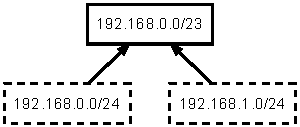
\includegraphics{figures/cidr_agg_adj.pdf}}
    \label{fig:cidr_agg:adj}}
    \subfigure[Aggregation by withdrawing more-specific prefixes (dashed boxes)
    covered by a less-specific prefix (solid box).]
    {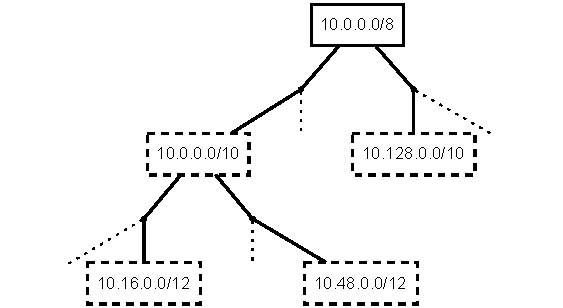
\includegraphics{figures/cidr_agg_cover.pdf}
    \label{fig:cidr_agg:cover}}
\caption{Aggregation approaches under CIDR addressing}
\label{fig:cidr_agg}
\end{centering}
\end{figure}

With the specification of classless network addresses codified in the CIDR
standard, the Border Gateway Protocol was updated to support this new method of
representing networks in the context of network reachability information. The
new version of the protocol, version 4 (sometimes referred to as BGP4), was
specified in 1994 \cite{rfc1654}.

The deployment of BGP4 required software and sometimes hardware upgrades to
routers. BGP4-speaking routers were not compatible with BGP3-speaking routers,
as the previous version of the protocol did not support CIDR. This required
some routers to speak both BGP4 and BGP3 to respective neighbors during the
transition period to BGP4. Nevertheless, the transition was relatively rapid in
terms of ``Internet time'', taking about 2 years \cite{Li:2011vn}, and was
strongly motivated by the relief in stress from routing table growth that many
network operators had been facing. According to \cite{rfc1773}:

\begin{quote} BGP-4 was rushed into production use on the Internet because of
the exponential growth of routing tables and the increase of memory and CPU
utilization required by BGP.  As such, migration issues that normally would
have stalled deployment were cast aside in favor of pragmatic and intelligent
deployment of BGP-4 by network operators.
\end{quote}

Even with the deployment of BGP4-speaking routers, aggregation did not
automatically occur by the agency of software running on the routers. Instead,
network operators needed to determine that their assigned address blocks were
aggregable and then announce these aggregates ``by hand''. This did not always
occur, especially for operators and a community that was used to speaking in
terms of classful addresses. Thus, even with the necessary condition of BGP4
routers deployed, the potential savings through aggregation was not realized
until network operators acted explicitly to aggregate their route
advertisements and the reduce number of routing table slots they were
consuming. It was this realization that motivated the creation of the CIDR
Report in the mid-1990s.

\subsection{The CIDR Report}

The CIDR Report presents a summary of interesting routing table behavior
related to routing table growth. The report contains a number of sections which
have varied slightly over time, but it has always contained an overall summary
of the size of the routing table over the past week, as well as the
\emph{aggregation report}, which is of greatest interest for this thesis. The
CIDR Report is published via email every Friday to the major mailing lists that
network operators participate in, including NANOG and similar lists in regions
outside of North America. A recent CIDR Report is shown in Appendix
\ref{chap:cidr_reports}, with an excerpt of the aggregation report shown below
in Figure \ref{fig:ex_cidr_report}.

\begin{figure}
\lstset{basicstyle=\scriptsize\ttfamily\fontsize{9}{9}\selectfont}
\begin{lstlisting}[frame=trlb]
Aggregation Summary
The algorithm used in this report proposes aggregation only
when there is a precise match using the AS path, so as
to preserve traffic transit policies. Aggregation is also
proposed across non-advertised address space ('holes').

 --- 12Nov10 ---
ASnum    NetsNow NetsAggr  NetGain   % Gain   Description

Table     340755   208585   132170    38.8%   All ASes

AS6389      3751      407     3344    89.1%   BELLSOUTH-NET-BLK -
                                               BellSouth.net Inc.
AS4323      4556     1679     2877    63.1%   TWTC - tw telecom holdings,
                                               inc.
AS6503      2001      433     1568    78.4%   Axtel, S.A.B. de C.V.
AS19262     1780      316     1464    82.2%   VZGNI-TRANSIT - Verizon Online
                                               LLC
AS4766      1728      575     1153    66.7%   KIXS-AS-KR Korea Telecom
\end{lstlisting}
\caption{An excerpt from the 12 November 2010 CIDR Report}
\label{fig:ex_cidr_report}
\end{figure}

With each week's CIDR Report, the aggregation report identifies the 30 ASes
announcing the most aggregable routes and thus consuming the most slots in the
global routing table that are unnecessary for the expression of routing policy.
For the purposes of the aggregation report, an aggregable route is a route
whose withdrawal would not cause a change in routing policy from the CIDR
Report's BGP vantage point.

Elements of the CIDR Report, and in particular the aggregation report, date
back to approximately 1994-1995 when it was implemented by Cisco Systems
employee Tony Bates. Bates was a member of the IETF's CIDR Deployment (CIDRD)
working group, and the report was conceived to educate and motivate networks
about the the transition to from classful to CIDR-aggregated route
announcements with the advent of BGP4. The earliest reports available on the
Internet date back to 1994, when it was referred to as the ``Top 10''
report\footnote{\url{ftp://ftp.ietf.org/ietf-online-proceedings/94jul/area.and.wg.reports/ops/cidrd/cidrd.bates.slides.ps}}.

In mid-1996 the CIDRD group wound down\footnote{
\url{ftp://ftp.ietf.org/ietf/cidrd/cidrd-minutes-96jun.txt}}, and Tony
transitioned the report to the NANOG mailing list. The first report still
accessible on the Internet, collected from the NANOG mailing list archives
\cite{NANOG} dates from September 1996, when the report was briefly called the
``Top-50'' report before being renamed as the ``CIDR Report''. The report as
originally conceived and implemented by Tony Bates was used until 23 August
2002. Geoff Huston then took responsibility for the report on 30 August 2002,
producing a similarly-formatted report but with a new implementation that was
developed without consulting Bates' source code \cite{Huston:2011ys}. The CIDR
Report's vantage points over time are in the table below\footnote{The potential
importance of vantage point selection is discussed further in Chapter
\ref{chap:discussion}.}. The CIDR Report is still published every Friday (North
American time zones) and has maintained a remarkably similar format over the 14
years where it can be observed on the NANOG mailing list.

\savenotes
\begin{table}[h]
    \begin{center}
    \small
    \begin{tabular}{c | c | c}
        AS number & AS Name & Date effective \\
        \hline
        AS 5413 & Xara.net (at MAE-East) & 17 September 1996 \\
        AS 5413 & GX Networks & 15 June 2001 \\
        AS 6447 & Route Views & 30 August 2002 \\
        AS 4637 & REACH & 11 October 2002 \\
        AS 2.0\footnote{AS 2.0 is not visible in the routing table, but peers
        with AS 4777 and AS 4608 \cite{Huston:2011ys}.} & APNIC R\&D & 20 July
        2007 \\
    \end{tabular}
    \vspace{1em}
    \caption{CIDR Report vantage point ASes over time}
    \label{table:cr_vantage_points}
    \end{center}
\end{table}
\spewnotes

\subsection{The aggregation report}

The purpose of the aggregation report is to identify ASes announcing routes
that could be more efficiently announced via aggregated route announcements
without altering expressed routing policy. In the specific context of the CIDR
Report, routing policy is simplified to mean inter-AS connectivity, captured
via the AS\_PATH for a given prefix. This is important for multihoming and some
forms of traffic engineering, where its necessary to announce more specific
prefixes in addition to the covering prefix to allow traffic to be spread
across multiple upstream providers instead of just taking the best route to the
covering prefix. Without considering the fact that there is variation in one or
more upstream ASes in the AS\_PATH, these prefixes would be considered
deaggregated even though they must be announced this way to achieve the desired
routing policy.

Given this desire to respect routing policy, the aggregation report considers a
prefix aggregable with another prefix if and only if the AS\_PATHs match
exactly. Aggregation is performed via the two approaches described earlier. The
aggregation report also apparently aggregates across an adjacent ``hole'', or
unannounced block, if there is no prefix below it. While this generally makes
sense, it is potentially over-optimistic in that it does not consider RIR block
allocations and the holes that may result from a block being allocated but
unadvertised\footnote{Unadvertised address blocks may be found in cases where a
provider wishes to advertise internal infrastructure using globally unique
addresses but not offer it as accessible to the public Internet}.

The number of advertised, aggregated, and withdrawn prefixes are totaled
against the AS originating each of the prefixes, and these figures are exported
to generate the CIDR Report. An example of the slightly more general CIDR
Report that is emailed to network operators was shown earlier in figure
\ref{fig:ex_cidr_report}, and an excerpt of the more detailed CIDR Report
available on the web is shown in Figure \ref{fig:ex_cidr_report_detail}.

\begin{figure}
\lstset{basicstyle=\scriptsize\ttfamily\fontsize{7}{7}\selectfont}
\begin{lstlisting}[frame=trlb]
Aggregation Report: Aggregation using AS prepended PATH

Report prepared at Sat, 13 Nov 2010 04:11:55 UTC+1000, using data obtained within AS0.6447

The report may include routes internal to AS0.6447, and may also include routes
that are accepted from adjacent AS's and marked ``NO EXPORT''. The report also
does not take into account conditions local to each origin AS in terms of policy
or traffic engineering requirements. As an aggregation guide, this report is a
very approximate guide at best.

AS list, ordered by net reduction in advertisements

AS            AS Name                                      Current  Wthdw  Aggte  Annce Redctn       %
              Routing Table                                 347822 174358  29764 203228 144594  41.57%
AS6389        BELLSOUTH-NET-BLK - BellSouth.net Inc.          3755   3526     53    282   3473  92.49%
AS4323        TWTC - tw telecom holdings, inc.                4555   3501    461   1515   3040  66.74%
AS19262       VZGNI-TRANSIT - Verizon Online LLC              1782   1643    144    283   1499  84.12%
AS4538        ERX-CERNET-BKB China Education and Research N   1670   1428     44    286   1384  82.87%
AS6503        Axtel, S.A.B. de C.V.                           2003   1534    258    727   1276  63.70%
AS4766        KIXS-AS-KR Korea Telecom                        1866   1315    122    673   1193  63.93%
\end{lstlisting}
\caption{An excerpt from the detailed 12 November 2011 CIDR Report}
\label{fig:ex_cidr_report_detail}
\end{figure}

In these figures, `current' or `netsnow' refers to the total number of prefixes
currently announced by the AS. `withdrawn' refers to the number of prefixes
that were able to be withdrawn after perfect aggregation. `aggregated' refers
to synthesized aggregate prefixes created by covering two adjacent prefixes.
`announced' or `netsaggr' refers to total number of prefixes announced by the
AS after maximum aggregation, and `reduced' or `netgain' refers to the total
number of prefixes saved by the aggregation process; in other words, reduced is
current less announced. ASes appear on the CIDR Report in order by decreasing
netgain.

% One benefit of coding the authoritative CIDR Report emails by hand was that
% it enabled observation of changes in the CIDR Report's BGP data vantage point
% and implementation over time, as well as the transition of stewardship of the
% report.

% \begin{verbatim}
% 	(example from email to geoff huston)
%
% 	Let's say peer A (AS 30) sees:
%
% 	10.0.0.0/8      30 20 10
% 	10.0.0.0/9      30 20 10
% 	10.128.0.0/9    30 20 10
%
% 	and peer B (AS 40) sees:
%
% 	10.0.0.0/8      40 10
% 	10.0.0.0/9      40 30 20 10
% 	10.128.0.0/9    40 30 20 10
%
% 	If you were to consider both peer's views, then you could aggregate 10/8's
% 	more specifics according to peer A but not according to peer B, and I was
% 	wondering how your algorithm decided whether 10/8's more specifics were
% 	aggregable for the CIDR Report?
%
% 	In the case where you use the router's best path for a given prefix
% 	which is what it sounds like from your answer to my question about MOAS
% 	prefixes, I assume you might see something like this for the above
% 	prefixes:
%
% 	10.0.0.0/8      40 10
% 	10.0.0.0/9      30 20 10
% 	10.128.0.0/9    30 20 10
% \end{verbatim}

% As noted in the previous section about BGP network operations, a number of
% routing policy objectives are implemented via BGP using different aspects of
% the protocol. Some of these are visible via the AS\_PATH, while others are
% not.  Thus, the CIDR Report may not perfectly avoid altering intentional
% routing policy that's not captured via the AS\_PATH.
%
% Other potential problems include the fact that the provider of the view for
% the CIDR Report may present a slightly different view than they export---i.e.
% they send their unfiltered RIB best paths, which may result in the use of
% non-operational routes for generating the CIDR Report. Similarly, while the
% attribution of behavior to the origin AS generally makes sense, it's
% conceivable that route leaks/etc. may be caused by peers or upstream
% providers that do not obey BGP communities/no-export/etc. or who send this
% information to the CIDR Report vantage point in spite of it being filtered
% for actual operations. (Somehow explain that I expect Geoff Huston is
% competent enough to have a ``good view'' of the routing table, but that these
% are dilemmas regardless due to BGP) These and other potential dilemmas
% regarding the measurement and ground truth of interdomain routing behavior
% are discussed in the later discussion chapter.
%
% NOTE: Geoff's policy of aggregating holes should prevent gaming (if only
% people cared enough to game the system) by advertising non-adjacent blocks

\section{Coordinating Internet Operations}

A hallmark of the Internet, especially in contrast to comparable telephony
networks, is its lack of regulation or centralized management. The very name of
the fundamental entities in interdomain routing---\emph{autonomous}
systems---suggest that networks are independent and free to do as they please.
Indeed, the Internet is a system where network operators, the individuals and
organizations that control infrastructure, can ``vote with their feet'' without
external intervention. Despite this autonomy, however, there is also a need for
coordination in key areas in order to facilitate interoperability and globally
unique identifiers---collective benefits that make the Internet better for
all.

Internet coordination was performed relatively casually in the early days of
the Internet as a DARPA project, and a number of these roles have evolved into
more formal organizations. Formal coordination of unique and high-value
resources---the Internet address space and the domain name system---has been
institutionalized in IANA and the Regional Internet Registries, and the
Internet Corporation for Assigned Names and Numbers (ICANN), respectively.
These organizations have established policy processes and engage stakeholders
in an effort to govern the resources they are responsible for in an effective
and legitimate way. Stakeholders in this space include governments, domain name
registry and registrar operators, trademark owners, Internet businesses and
service providers, policy advocates, and consumers.

Slightly less formal are the organizations responsible for technical
coordination of the Internet. The organizations involved in this space, which
include the Internet Architecture Board (IAB) and the Internet Engineering Task
Force (IETF), are charged with developing technical standards for the Internet
in a fair and open way, in order to improve interoperability and technical
coordination amongst network operators and equipment vendors. The IETF is
responsible for the well known ``Request for Comments'' (RFC) series of Internet
drafts and standards. While once the domain of researchers and network
operators, the IETF participants have grown to include representatives from
network hardware and software vendors who now play a large role in the IETF
\cite{Li:2011vn}.

The least formal level of Internet coordination occurs at the operations level.
This refers to the coordination between interconnecting service providers that
is necessary in order to implement that interconnection, as well as to solve
other problems or work towards developments that are only manifest in
operational Internet infrastructure. Most interconnection and bilateral dealing
between ISPs is organized through contracts and business relationships (though
some activities also take place through more informal channels mediated by
personal identity and reputation), whereas collective coordination and
operational problem solving typically occurs within Internet operator
communities.

\subsection{Internet Operator Communities}

The North American Network Operators' Group (NANOG) is the canonical example of
an Internet operator community. Emerging out of a previous group of NSFNET
operators called ``Regional Techs'', the group holds large (400-600 person)
meetings three times a year in cities across the United States and Canada for
operators to meet and share knowledge (``clue'') while also building business
and personal relationships. In addition, and perhaps more significant, is the
NANOG mailing list, which is composed of approximately 10,000
participants\footnote{The most recent statistics are from December 2009:
\url{http://nanog.org/mailinglist/liststats/2009stats.php?mon=dec}} and is
commonly used for making contact with other operators about operational issues,
or discussing technical problems. While not all North American networks
participate in this community, it is popular and common amongst medium and large
Internet networks. The norms and attitudes of NANOG and the individuals that
participate in it are generally cooperative and meritocratic
\cite{Mathew:2010ly}, in keeping with the ethos of the early Internet
\cite{Abbate:2000ve}.

NANOG is nominally limited to the North American continent, but it is also the
preeminent operator mailing list and community worldwide, and so attracts
participation from major operators and clueful individuals from organizations
in other regions. There are also other geographically bounded communities that
serve a similar role to NANOG in other regions. Many of these are coupled
together with the RIR role in each locale. This suggests that shared language
or culture, and the ability to meet in person are important for
the activities of network operator groups, even if most participate only via
mailing lists.


